\section{Stehende Wellen}

\subsection{Terminologie}

Eine \textbf{stehende Welle} ist eine Welle, bei der Orte maximaler Auslenkung (oder minimaler Auslenkungen) sich \textbf{nicht fortbewegen}. 

\smallskip

\begin{itemize}
	\item Ort- und Zeitabhängigkeit sind separiert 
	\item Die Welle bewegt sich nicht im Raum ('Muster bleibt stehen') 
\end{itemize}

$$ \boxed{ \xi(x, t) = \xi_0 \cdot \cos(\omega t) \cdot \cos(k x) }  \qquad \quad \text{ \textrightarrow\ } \sin() \text{-Terme sind auch erlaubt!} $$

\medskip

\begin{outline}
    \1 Orte, wo die Welle für alle Zeit $= 0$ ist heissen \textbf{Wellenknoten} \\
        \textrightarrow\ \textbf{Zwei benachbarte Knoten sind $\boldsymbol{\frac{\lambda}{2}}$ auseinander}
    \1 Orte, wo die Welle eine maximale Auslenkung erreicht, heissen \textbf{Wellenbauch} \\
        \textrightarrow\ \textbf{Zwei benachbarte Bäuche sind $\boldsymbol{\frac{\lambda}{2}}$ auseinander}
\end{outline}



\subsection{Entstehung von stehenden Wellen}

\begin{center}
    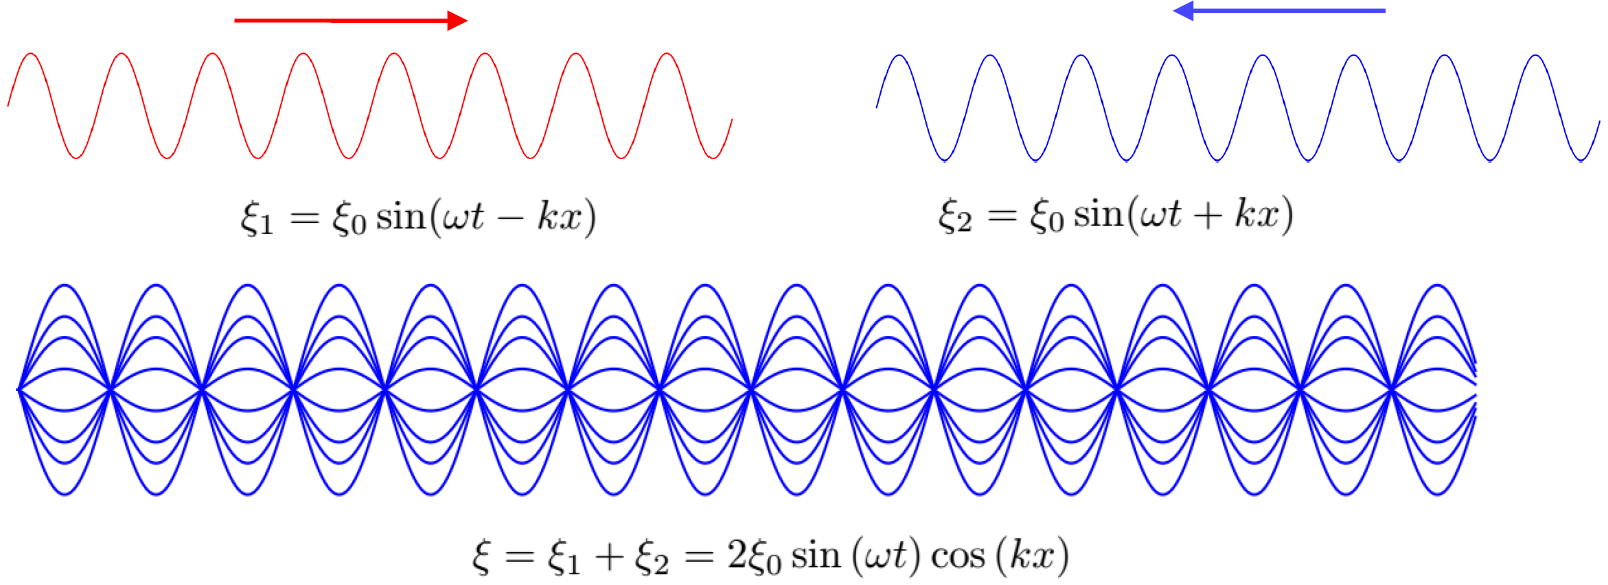
\includegraphics[width=0.85\columnwidth]{images/stehende_wellen.png}
\end{center}



\subsection{Prinzip von Huygens}

\begin{minipage}[t]{0.4\columnwidth}
    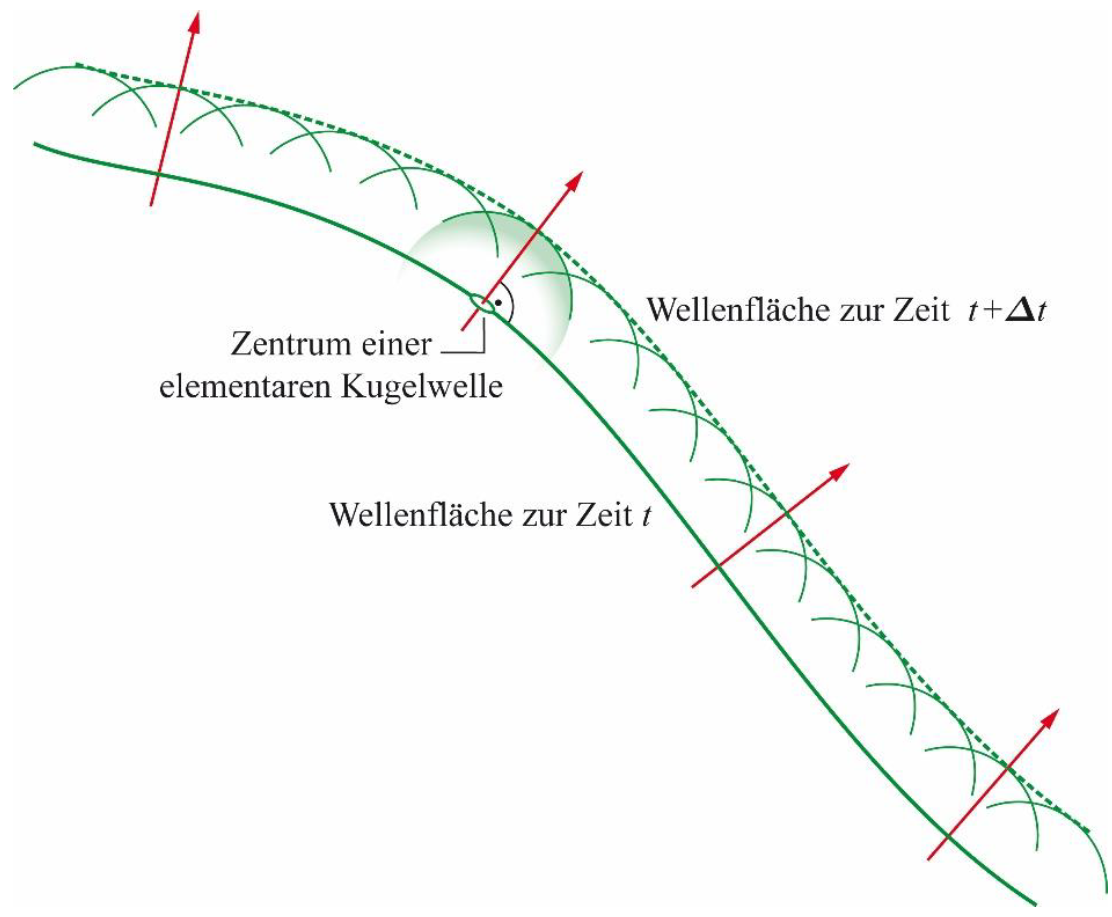
\includegraphics[width=\columnwidth, align=t]{images/huygens.png}
\end{minipage}
\hfill
\begin{minipage}[t]{0.55\columnwidth}
    \raggedright
    Jedes Flächenelement auf einer Wellenfläche kann als Zentrum einer Kugelwelle betrachtet werden. \\
    Die Wellenfläche zu einem späteren Zeitpunkt ist die Einhüllende all dieser Elementarwellen.
\end{minipage}


\subsection{Eigenschwingungen -- 1D}

\begin{minipage}{0.3\columnwidth}
    $$ \boxed{ f_n = \frac{n}{2 \, l} \cdot u = \frac{u}{\lambda_n} } $$
\end{minipage}
\hfill
\begin{minipage}{0.66\columnwidth}
    $$ \boxed{ \text{Auslenkung = 0: }\quad k_n \cdot l = n \cdot \pi } $$
    $$ \boxed{ \text{Auslenkung max: }\quad k_n \cdot l = \frac{\pi}{2} + n \cdot \pi } $$
\end{minipage}


\subsubsection{Saite}

\begin{itemize}
	\item Reflexion an einer Grenzfläche $\rightarrow$  Stehende Welle 
	\item Stehende Welle muss in vorhandenen Raum passen \textrightarrow\ Geometrische Bedingung 
	\item \textbf{Knoten an beiden Enden} 
\end{itemize}

\smallskip

\begin{minipage}{0.48\columnwidth}
    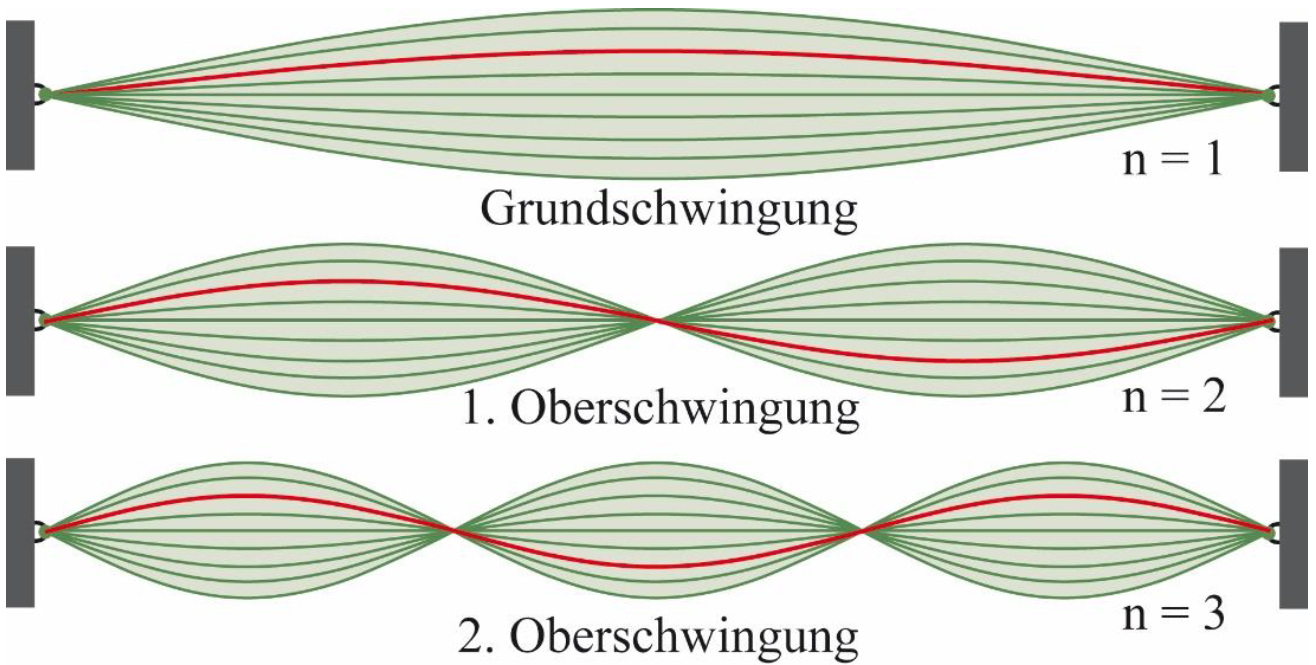
\includegraphics[width=\columnwidth]{images/saite.png}
\end{minipage}
\hfill
\begin{minipage}{0.48\columnwidth}
    $$ \boxed{ \xi = \xi_0 \, \sin(\omega t) \cdot \sin(k x)  } $$
    $$ \boxed{ \text{Auslenkung = 0: } k_n \cdot l = n \cdot \pi } $$
    $$ \boxed{ f_n = \frac{u}{\lambda_n} = \frac{n}{2 \, l} \cdot u = \frac{n}{2 \, l} \sqrt{\frac{F}{\rho \cdot A}} } $$
\end{minipage}

\renewcommand{\arraystretch}{1.2}
\begin{ctabular}{clc}
    $k_n$       & Wellenzahl                & $[k_n] = \frac{1}{\meter}$        \\
    $l$         & Länge der Saite           & $[l] = \meter$                    \\
    $u$         & Wellengeschwindigkeit     & $[u] = \frac{\meter}{\second}$    \\
    $\lambda_n$ & Wellenlänge               & $[\lambda_n]= \meter$             \\
    $n$         & Ganze Zahl                & $[n] = 1$                         \\
    $\omega$    & Kreisfrequenz             & $[\omega] = \frac{\rad}{\second}$ \\
    $A$         & Querschnitt der Saite     & $[A] = \meter\squared$
\end{ctabular}
\renewcommand{\arraystretch}{1}


\subsubsection{Pfeiffen}

\begin{minipage}[t]{0.48\columnwidth}
    \paragraph{Offene Pfeiffe}
    Länge $l = \frac{\lambda}{2}$

    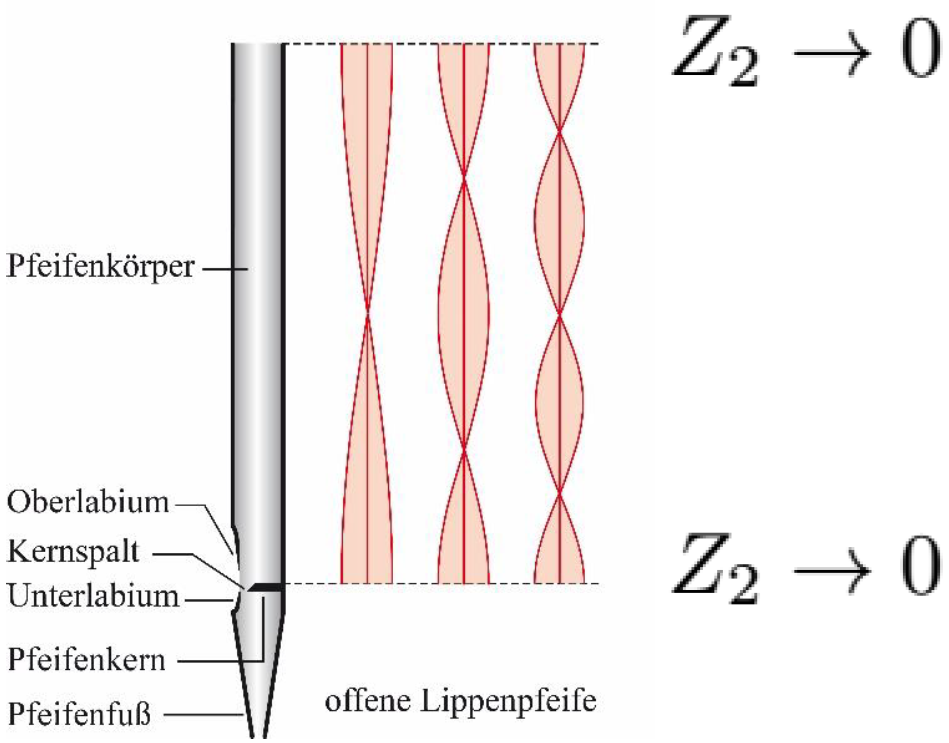
\includegraphics[width=0.85\columnwidth, align=t]{images/offene_pfeiffe.png}

    \smallskip

    Auslenkung an Enden: \\
    Wellenbauch
\end{minipage}
\hfill
\begin{minipage}[t]{0.48\columnwidth}
    \paragraph{Gedackte Pfeiffe}
    Länge $l = \frac{\lambda}{4}$

    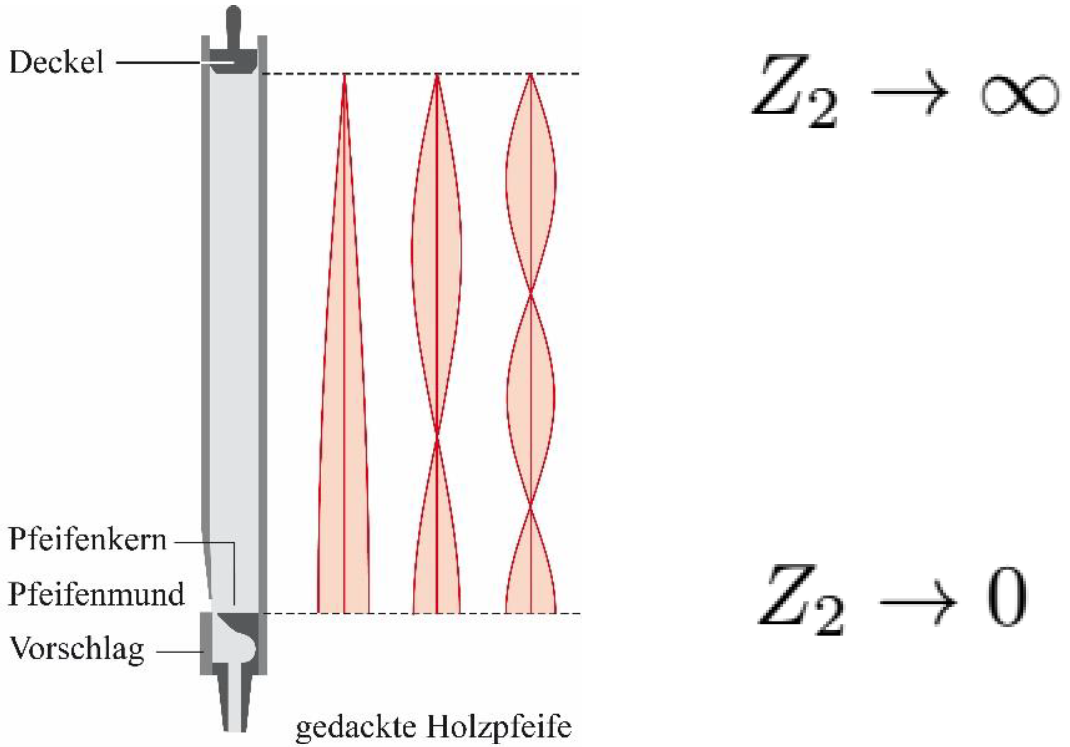
\includegraphics[width=0.9\columnwidth, align=t]{images/gedackte_pfeiffe.png}

    \smallskip

    Auslenkung offenes Ende: \\
    Wellenbauch \\
    Auslenkung gedacktes Ende:\\
    Knoten (max. Auslenkung)
\end{minipage}


\subsection{Eigenschwingungen -- 2D}

\subsubsection{Rechteckige Membrane}

\begin{minipage}{0.3\columnwidth}
    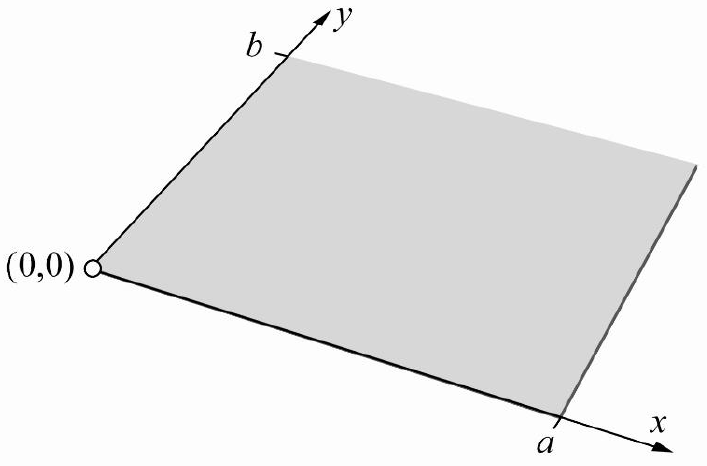
\includegraphics[width=\columnwidth]{images/membrane.png}
\end{minipage}
\hfill
\begin{minipage}{0.68\columnwidth}
    $$ \boxed{ \xi(x,y,t) = \xi_0 \, \sin(\omega t) \, \sin(k_x x) \, \sin(k_y y)  } $$

    $$ \boxed{ \text{Wellenvektor:} \quad  k = |\vec{k}| = \sqrt{k_x^2 + k_y^2}} $$

    $$ \boxed{ u^2 = \frac{\omega^2}{k^2}} $$
\end{minipage}

\medskip

\paragraph{Randbedingungen}

\begin{tabular}{l c c }
    Auslenkung = 0 &  $ \boxed{ k_x = \frac{n \, \pi}{a} }$ & $ \boxed{ k_y = \frac{m \, \pi}{b} }$
\end{tabular} 

